% Drawing 83/11-3 -- folder 83, batch 11, archive page 204 (PDF page 205).
% Transcription: Un cube en perspective ; trois sommets marqués $s_1$, $s_2$, $s_3$ autour d'un sommet $s$ cerclé ; chaque face visible porte une petite flèche circulaire (orientation).
% Kind: cube with oriented faces. Method 2 (schematic redraw from the facsimile). Status: ok.
% Notes: Cube; the vertex s (front top right) circled, s_1, s_2, s_3 around it (s_1 back top right, s_2 front top left, s_3 front bottom right); a small circular arrow on each visible face. Hidden edges faint.
% Coordinates: 1 unit = 1 mm = 1/100 of the crop width (bbox in page fractions: [0.12, 0.12, 0.33, 0.27]).
% Redrawn by Claude (claude-opus-5-5), issue #73, 2026-11-07; not checked by a human; not compiled (no TeX in the session).
% Rights: reproduces part of the work -- behind RENDER_TRANSCRIPTS, never published by itself.
\documentclass[tikz,border=3pt]{standalone}
\usepackage{amsmath,amssymb}
\usetikzlibrary{patterns,arrows.meta}
\tikzset{pencil/.style={black!45}, struck/.style={black!35}, mark/.style={circle,draw,inner sep=1.3pt}, pt/.style={circle,fill,inner sep=0.9pt}, opt/.style={circle,draw,fill=white,inner sep=1.1pt}}
\begin{document}
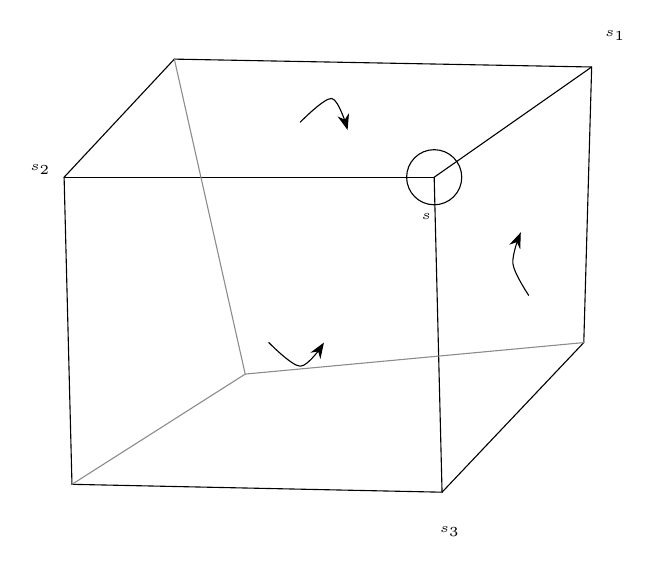
\begin{tikzpicture}[x=1mm,y=1mm,line cap=round,line join=round,font=\scriptsize]
\draw (18,-37) -- (65,-37);
\draw (65,-37) -- (66,-77);
\draw (66,-77) -- (19,-76);
\draw (19,-76) -- (18,-37);
\draw (18,-37) -- (32,-22);
\draw (32,-22) -- (85,-23);
\draw (65,-37) -- (85,-23);
\draw (85,-23) -- (84,-58);
\draw (66,-77) -- (84,-58);
\draw[pencil] (32,-22) -- (41,-62);
\draw[pencil] (41,-62) -- (84,-58);
\draw[pencil] (19,-76) -- (41,-62);
\draw (65,-37) circle[radius=3.5];
\node[inner sep=1pt] at (88,-19) {\tiny $s_1$};
\node[inner sep=1pt] at (15,-36) {\tiny $s_2$};
\node[inner sep=1pt] at (67,-82) {\tiny $s_3$};
\node[inner sep=1pt] at (64,-42) {\tiny $s$};
\draw[-{Stealth[length=2mm]}] plot[smooth, tension=0.55] coordinates {(48,-30) (52,-27) (54,-31)};
\draw[-{Stealth[length=2mm]}] plot[smooth, tension=0.55] coordinates {(44,-58) (48,-61) (51,-58)};
\draw[-{Stealth[length=2mm]}] plot[smooth, tension=0.55] coordinates {(77,-52) (75,-48) (76,-44)};
\end{tikzpicture}
\end{document}
